\documentclass[12pt]{article}
\usepackage[a4paper, total={6in, 8in}]{geometry}
\usepackage[utf8]{inputenc}
\usepackage[round]{natbib}
\usepackage{graphicx}
\usepackage{dblfloatfix}    % To enable figures at the bottom of page
\usepackage{rotating}
\usepackage{tikz}
\usepackage{authblk}
\usepackage{booktabs, tabularx}
\usepackage{amsmath}
\usepackage[input-decimal-markers=.]{siunitx}
\usepackage[english]{babel}
\usepackage{pdflscape}
\usepackage{setspace} \doublespacing
\usepackage{dcolumn,caption}
\usepackage{array, threeparttable} % to add footnotes to the tables
\setlength{\emergencystretch}{3em}
\captionsetup{skip=0.333\baselineskip}
\newcolumntype{d}[1]{D{.}{.}{#1}}
\newcommand\mc[1]{\multicolumn{1}{@{}c@{}}{#1}} % handy shortcut macro

\begin{document}

\title{The signaling role of skills endorsement for start-up teams' funding: an empirical study}
\date{\vspace{-3ex}}
\author{Arnauld Bessagnet \\ \footnotesize{LEREPS – Sciences-Po Toulouse, University of Toulouse – France} \\}

\maketitle \vspace{-1,5em}

\begin{abstract}
\noindent
Entrepreneurship research and signaling theory suggest that start-up teams' human capital has a signal-quality effect on how easily they can access financial resource from investors. Based on a sample of 514 software-based firms, we examine the signal effect of skills and expertise endorsement, a peer-reviewed relational measure of professional capabilities, and its influence on the amount of external funding received in early stage. Results show that investors favor start-up teams that have either a high level of competency or a high level of variety of skills, but only some at once. We discuss the implications of these findings for the research literature on digital entrepreneurship and venture capital. \newline

\begin{obeylines}
\noindent \footnotesize{}{\textbf{Keywords:} Skills, Entrepreneurship, Fundraising, Start-up Teams, Variety}
\noindent \footnotesize{\textbf{JEL Classification:} L22, L26, L85}
\end{obeylines}

\end{abstract}

\clearpage
\section{Introduction}

Start-up teams, i.e., group of individuals which possess attributes such as equity ownership, decision-making autonomy and entitativeness \citep{knight2020start}, are seen as vital agents in the development of cities, regions and countries, due to their role in the creation and growth of firms \citep{audretsch2001linking, autio2016entrepreneurship}. Acquiring financial resources from investors is a key factor in the survival and expansion of start-up teams \citep{rosenbusch2013does}, thus making the determinants of attracting such resources of great interest to researchers, practitioners, and policy makers \citep{EUcommission2015digital}. This is especially relevant in the digital economy, where low-resource-intensive systems offer investors new possibilities to multiplicte their return on assets since digital technologies can generate non-linear revenues in an efficient, predictable, and repeatable manner \citep{nambisan2017digital, sahut2021age}. This article contributes to the critical agenda by exploring the connection between start-up teams' human capital signals and their performance in a digital context, paying particular attention to external capital financing resource access.

Which start-up teams are funded and why are recurring themes in contemporary economic and entrepreneurial literature \citep{baum2004picking, beckman2007early, bernstein2017attracting, franke2006you, franke2008venture, kaplan2009should, plummer2016better, shane2002network}. [TEAM COMPOSITION AND CONSENSUS]

Highlighting the complexity of the effects of start-up teams' composition on investors’ evaluations \citep{ghassemiautomated}, research has found that individual qualities of founding members - such as education, work experience, and prior entrepreneurial endeavors \citep{shane2002network, hsu2007experienced} - and their social capital — the direct or indirect relationships that founding members have with investors, corporate partners, and other entities \citep{shane2002network, hsu2007experienced, huang2017resources} - act as a signal of venture quality and therefore is a determinant of financial resources acquisition. While these studies has yielded several important insights, this approach is problematic as investors nowadays draw on a wide range of other signals to assess the relevance of investing in a startup team. For instance, \citet{banerji2019startup} found that founders' number of followers on their LinkedIn profiles was the strongest predictor of the amount of funds raised. In the same vein, based on data available on Kickstarter crowdfunding webnsite, \citet{mollick2014dynamics} evidences that founders' Facebook connections help equity crowdfunding success and \citet{courtney2017resolving} show how third party online endorsements help firm attract fundings. Additionally, some social networks, such as LinkedIn and ResearchGate, allow users to endorse specific skills \citep{perez2016endorsement, wu2018analysis}. In the managerial literature, skill endorsement is considered a socially constructed online reputation and a way of self-presentation through which job seekers brand themselves to potential recruiters \citep{rapanta2017linkedin}. Concretely, it permits users to tag themselves with topics representing their area of expertise and have their connections provide social proof of their competence in that topic. Recently, researchers have considered skills and expertise endorsements data as valuable information for entrepreneurial studies and consider it as a reliable criteria in order to judge anperson’s knowledge authority \citep{reese2020should, sako2020scaling}. Nonetheless, research on the potential signaling effects of skills and expertise endorsement on early stage resource acquisition was left out by researchers. This study seeks to fill this gap by examining the role of skills and expertise endorsement in resource acquisition during the early stages of entrepreneurship. Drawing on the theory of signaling, we explore how social construction of peer-reviewed measures of professional capabilities can influence the ability of startup teams to acquire financial resources from investors.

Using data from a sample of 514 french software-based ventures listed on Crunchbase and BPI France combined with data from LinkedIn, company websites, and press articles, we constructed a unique dataset that includes what \citet{marvel2016human} call the "human capital investments" (i.e., common traditional signals used by investors such as years of education, professional experience, and previous founding experience) and "outcomes of human capital" (i.e., skills and expertise) of start-up teams. We analyze our statement in two stages. First, we examine the relationship between the level of skills and expertise endorsement of start-up teams and its impact on capital acquisitions in early-stage investment. Secondly, drawing from the cognitive distance model \citep{nooteboom2007optimal} and the cybernetics principles of requisite variety applied to the entrepreneurship literature \citep{ashby1957introduction, harrison2007s}, we assess the extent to which signals from startup teams' skills and expertise endorsements variety help the firm acquire capital. Following our claims, we find that investors favor start-up teams that have either a high level of competency or a high level of variety of skills, but not both at once.

This work contributes to the literature in three ways. Firstly, it expands upon previous investigations of the effect of human capital social media data on venture financing \citep{banerji2019startup, marvel2016human, mollick2014dynamics, reese2020should}. To the best of our knowledge, this is the first to explicitly examine the signaling impact of skills and expertise endorsements on resource acquisition. Secondly, this study builds upon the literature on signaling and new venture financing \citep{colombo2021use, drover2017review, klein2020start}. Lastly, this work demonstrates the utility of endorsements data for research, specifically to elucidate the dynamics of signals in entrepreneurship literature in early stage.

The paper is structured as follows. Section 2 reviews the literature on signaling theory for early-stage resource acquisition. Section 3 explains the data and methods used, and Section 4 presents key findings. Finally, section 5 concludes by discussing implications for theory and practice, noting the limitations of this study.

\section{Theoretical framework and hypothesis}

\subsection{Signaling theory for early-stage resource acquisition}

Literature on entrepreneurship has continually underscored the critical role of external financial resources for the survival and growth of new firms \citep{cooper1994initial}. Despite the numerous types of external financial sources obtainable to start-up teams \citep{drover2017review, klein2020start}, the majority of research has concentrated on the acquisition of capital from external investors, who provide financial capital in return for a stake in the firm's ownership. Nevertheless, securing external funding from external investors is a challenging task, with investors having difficulty predicting which teams will come out on top \citep{ghassemiautomated}, due to the inherent information asymmetries between them and entrepreneurs, or the lack of past financial results. In order to mitigate the information asymmetries, investors draw on quality-signals \citep{ko2018signaling, spence1978job, subramanian2022backing}, with signalling theory being particularly applicable in the digital context, where new digital technologies have transformed the nature of uncertainty inherent in entrepreneurial processes \citep{nambisan2017digital}.

Signaling theory posits that two parties take conscious and voluntary steps to reduce asymmetric information and perceived uncertainty between them, and this is done by focusing on the signals available to them \citep{spence1974market}. This concept has been used in various disciplines to provide insight into social selection problems when there is an absence of perfect information \citep{connelly2011signaling, colombo2021use}. Entrepreneurship scholars have found this concept to be beneficial as particular signals can diminish uncertainty about ventures' quality in the eyes of stakeholders, such as prestigious government grants \citep{islam2018signaling}, the enthusiasm and passion of the founders \citep{chen2009entrepreneur}, affiliations of the venture with other entities \citep{plummer2016better}, and the composition of the founders' team \citep{ko2018signaling}. Investors, similarly, use a variety of indicators to mitigate asymmetric information such as the founders' ties to others \citep{shane2002network}, their human capital \citep{beckman2007early}, social capital \citep{shane2002organizational}, and endorsements \citep{courtney2017resolving, janney2006moderating, plummer2016better}.

In the context of early-stage ventures, human capital of the start-up teams is considered to be a significant and prominent factor for investors to consider \citep{beckman2007early, ko2018signaling, matusik2008values}. This emphasis is due to the limited resources and small number of people responsible for formulating and carrying out strategies. According to the organizational theory perspective applied to the entrepreneurship field, the human capital composition of the start-up teams is believed to have an imprinting effect on the processes and operations of the firm \citep{packalen2007complementing}. This concept implies that past experiences, and therefore the underlying skills and experiences acquired meanwhile, can shape the present performance. Concretely, investors aim to reduce uncertainty about the quality of the firm by relying on the human capital and demographic characteristics of start-up teams such as their educational background or their functional skills because these are easily accessible quality-signals \citep{colombo2005founders, beckman2007early, eddleston2016you, plummer2016better}.

Extensive research has been conducted to explore the association between signaling and the acquisition of financial resources (see \citep{connelly2011signaling} and \citet{colombo2021use} for a review). However, to the best of our knowledge, no studies have examined the signaling role of skills and expertise online endorsement - a human capital data available on professional social networks that we consider as a reliable criteria in order to judge a person’s knowledge authority \citep{rapanta2017linkedin} - and financial resource acquisition in the early stages of venture creation. This gap in the literature is remarkable given that the level of uncertainty \citep{matusik2008values} and information asymmetry between the signal sender and receiver \citep{spence2002signaling} are most pronounced during this period. Therefore, any kind of quality-signals that help gain additional perspective and triangulate start-up teams data is welcomed by investors. At this juncture, a new venture typically has no track record of performance to rely on, yet must still find a way to convince stakeholders that it is a legitimate venture \citep{becker2015new}, and thus worthy of obtaining necessary resources, such as financial capital \citep{ko2018signaling}.

In the next sections, this paper investigates how investors might rely on human capital social media data signals to determine the potential of new firms they are considering investing in. To this end, we will focus on the signal effect of skills and expertise endorsement, a peer-reviewed relational measure of professional capabilities feature on LinkedIn, the world's largest professional online social network \citep{wu2018analysis}. This feature enables members to tag themselves with topics representing their areas of expertise and their connections to provide social proof via the endorsement of said member's competency in the topic.

\subsection{Signaling effects from start-up teams' level of skills and expertise endorsement}

Entrepreneurship researchers have extensively explored what start-up teams' characteristics enable them to access external funding \citep{roure1990predictors}. The focus on start-up teams stems from the fact that most entrepreneurial initiatives are run mainly by groups of individuals rather than by lone individuals \citep{klotz2014new}. Such characteristics include the teams' social capital \citep{shane2002network}, the team's demographics and size \citep{eisenhardt1990organizational}, the teams' match with an investor's characteristics \citep{aggarwal2015evaluating}, the industry environment \citep{townsend2015turning} or the investor's experience \citep{franke2008venture}. However, in the context of early-stage ventures, human capital of the start-up teams is maybe the most significant and prominent factor for investors to consider \citep{beckman2007early, ko2018signaling, matusik2008values}.

In the literature, skills are considered human capital outcomes and refer to agents’ "observable applications or know-how related to a domain" \citep{becker1964human, marvel2016human}. In this this study, conformed to the human capital literature applied to the entrepreneurial field, we postulate that start-up teams with higher levels of skills have a greater propensity to reach specific entrepreneurial milestones, elicit greater investor confidence, and a greater likelihood of attracting external financial capital. Indeed, it has been shown that higher levels of skills enable founders to take greater risks and demonstrate proactive behavior \citep{becherer1999proactive}, allowing them to optimize business opportunities \citep{shane2000promise, chandler1994founder}. Additionally, the acquired skills enable entrepreneurs to make full use of the available technological tools in a digital context \citep{nambisan2017digital}, enabling them to better understand and differentiate their offerings through the introduction of new technologies and disruptive products \citep{marvel2007technology}. Moreover, a high level of skill proficiency can help entrepreneurs to obtain resources complementary to financial resources, which is an issue for many firms in the early stages of development \citep{beckman2007early}. Finally, developing skills and knowledge is a prerequisite for further entrepreneurial learning and helps business owners acquire additional skills and knowledge that will help their firm grow \citep{hunter1986cognitive}.

Therefore, for all these reasons, we propose that a high level of skills and expertise endorsements within a start-up team enhances the quality of the signal intended for investors looking to engage financially in the early stages. The investors are alterted by this signal because it suggests that higher skill levels may translate into future success. Thus, we hypothesize the following: \\

\noindent \textit{H1: Start-up teams with greater skills and expertise endorsement levels will get more fundings from investors}

\subsection{Signaling effects from start-up teams' variety of skills and expertise endorsement}

In this study, we consider not only the level of skills but also their variety \citep{harrison2007s}. Skills' variety in a start-up team matters because the success of entrepreneurial initiatives is often the result of teamwork and collective endeavors, which require the combination of knowledge, the synergy of abilities, and the collaboration of multiple individuals \citep{klotz2014new}. This paper argue that start-up teams with a wide range of skills and expertise endorsement have a greater chance of acquiring investors due to two key reasons.

The first reason relates to the decision-making process. The underlying argument is that groups with various skills take better decisions because they have access to more information \citep{hong2001problem}. Therefore, the solutions to new issues encountered during entrepreneurial cycles might result from recombining existing knowledge under new forms. A meta-analysis conducted by \citet{jin2017entrepreneurial} suggests that an entrepreneurial teams endowed with a varied skill set are more likely to use various market entry, internationalization or innovation strategies \citep{boeker1989strategic}. This implies that start-up teams with diverse skills are in a better position to make high-quality decisions, thus increasing their chances of success. Consequently, investors may use start-up teams' skills variety as a signal to assess their future performance, which can significantly impact the probability of receiving investments.

The second reason related to the connection between start-up teams' skills and expertise variety and their social capital. The literature demonstrates that the social capital of a start-up team has the capacity to act as control for information asymmetries. Indeed, \citet{huang2017resources, shane2002organizational} posit that the presence of a social connection between start-up teams and investors can reduce the informational gap between them. Specifically, \citet{shane2002network} infer that social capital play a role in connecting start-up teams to potential investors and facilitating fundraising. Additionally, \citet{hoenig2015quality} suggest that the social capital of a start-up team is utilized by investors to triangulate the quality of the firm and the composition of start-up teams and their relationships (alliances) are used as indicators of quality by investors \citep{plummer2016better, semrau2014exactly}. Following these rationales, if a start-up team's variety of skills endorsements is the result of different social capital and given that capital influences the start-up teams' ability to raise funds from investors, start-up teams with diverse skills might therefore raise more funds than less diversed ones. Thus, we hypothesize the following: \\

\noindent \textit{H2: Start-up teams with greater skills and expertise endorsement variety will get more fundings from investors} \\

The past two rationales invite us to think that having high both highly skilled individuals and a high levels of variety within a startup team is beneficial for firm performance. However past findings suggest that adding more human capital to a start-up team does not necessarily translate into greater success \citep{pierce2013too}.

Indeed, if empirical entrepreneurship investigations propose that a particular level of expertise stimulates the detection of new business \citep{shane2000promise, marvel2016human}, elevates the likelihood of generating remarkably new and commercially viable services, and boosts the chances of obtaining external funding \citep{beckman2007early, marvel2007technology}, conversely, cognitive and social psychology findings indicate that highly skilled individuals across various fields tend to possess greater cognitive inelasticity and greater cognitive distance \citep{nooteboom2007optimal}. Cognitive inelasticity arises from the prolonged exposure to a specific field, which engenders a cognitive model that adheres to the prevalent logical pattern of that field. Although cognitive inelasticity can lead to greater determination, it can also diminish one's receptiveness to entirely distinct logics and approaches, hinder communication within a start-up team, and limit the team's exploitation of its knowledge. Therefore, the dangers of cognitive inelasticity are more probable and particularly menacing when two or more persons share a high cognitive distance.

Cognitive distance denotes the degree to which two or more people have created distinct cognitive models or belief systems \citep{nooteboom2007optimal}. High cognitive distance may create obstacles to communication and collaboration within a startup team and limit openness to innovative business models, such as pivoting \citep{kirtley2020pivot}. Though any two individuals inherently have some degree of cognitive divergence, those who share comparable abilities and fields of expertise tend to have lower cognitive distance, as they are more likely to be familiar with each other's cognitive models and therefore can establish the essential mutual trust for a social group's effective functioning. Conversely, those with completely different areas of expertise are more prone to possess divergent outlooks and knowledge, thereby increasing their cognitive distance. As a result, this reduces the quality of their interactions, decisions, and ability to interact effectively. Since the adverse impacts of cognitive distance are more pronounced when group members have firmly established cognitive models and entrenched opinions and positions (i.e., when they are cognitively inflexible), startup teams comprised of highly skilled individuals from different domains may not fully exploit the benefits of their varied skill sets, information, and social capital. Consequently, we put forth the following hypothesis: \\

\noindent \textit{H3: Start-up teams' skill and expertise endorsement variety impact negatively the positive effect of level of skill and expertise endorsement on the funds raised} \\

Our formal hypotheses (H1, H2, H3) conform with the proposed model presented in Figure \ref{Figure1}

\begin{figure*}[!b]
  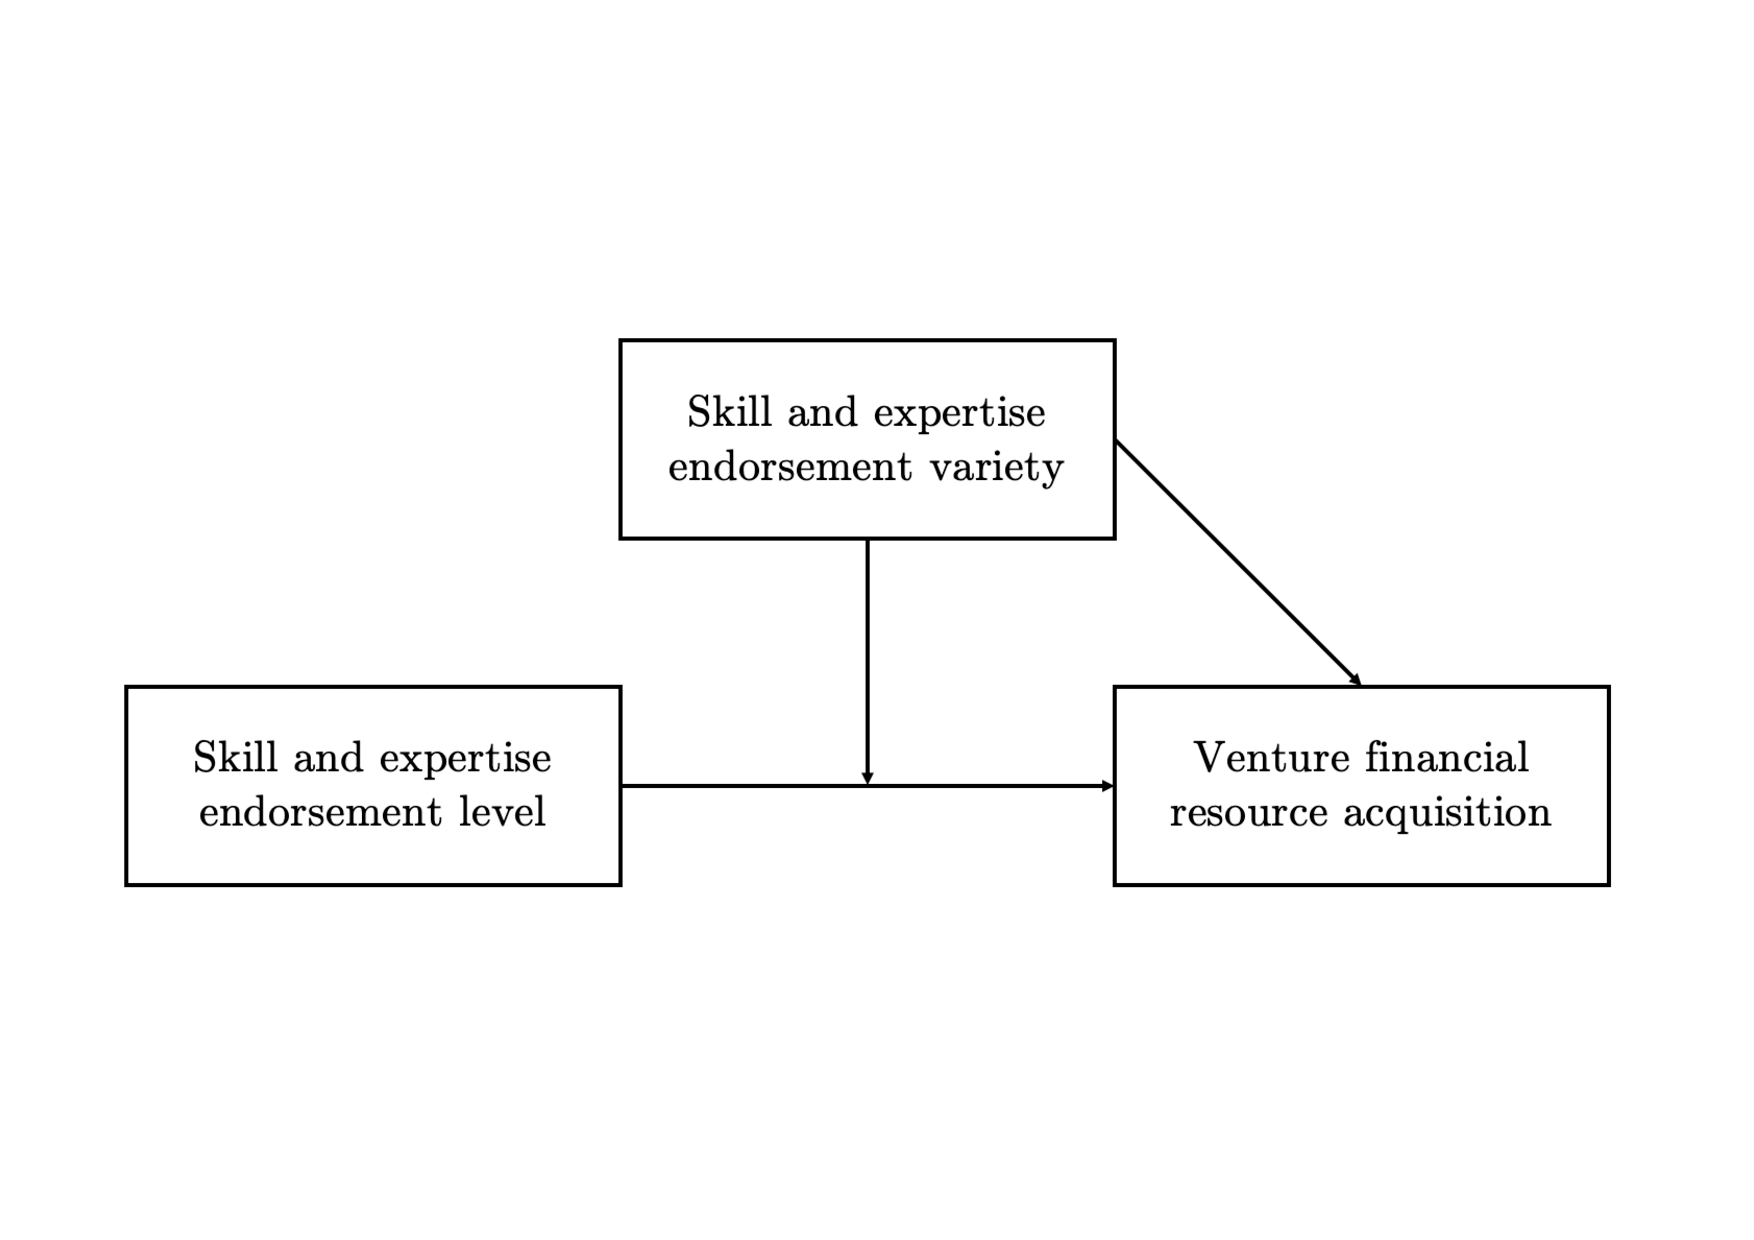
\includegraphics[width=\linewidth, scale=0.5]{model.pdf}
  \caption{Research Model}
  \label{Figure1}
\end{figure*}

\section{Methodology}

\subsection{Data sources and collection process}

To test our hypotheses, we built a dataset with information on firms, their fundraising activities, and granular information on the skill and expertises of start-up teams' members. Table 1\label{table1} lists our empirical variables, definitions, and sources. Table 2\label{table2} provides the general statistics and distribution across sectors. Table 3\label{table3} provides the descriptive statistics of the fundraising activities of the 514 firms in our sample. We detail the collection process below. \\

INSERT TABLES 1, 2 AND 3 HERE. \\

First, we draw on Crunchbase, and BPI France databases as a starting point. The first database follow the evolution of global firms benefiting from venture capital financing. The second is a French state database that lists French-based digital and innovative firms. These databases provide information on the firm’s headquarters, founders’ names, fundraising activity, business models, and date of foundation. We collected this data in March 2020 and kept firms that (i) were founded between 2011 and 2018, (ii) had their headquarters in the Metropolis of Greater Paris (France), (iii) were independent (no subsidiaries), (iv) operated in business-to-business markets and (v) used a scalable business model in the software industry. From these filters, we ended up with 514 firms. We chose to study software-based firms with scalable business models (i.e., software-as-a-service, marketplaces, and platforms) because they echo the efficient, predictable, and repeatable systems that offer investors new opportunities due to the non-linear revenues of digital technologies \citep{nambisan2017digital}. Unlike traditional software licenses that require installers, scalable business models are hosted in the cloud, require little infrastructure, are searchable using a browser, and are delivered over the Internet with or without a subscription- based revenue logic. We also chose the period 2011-2018 because it coincides with the mass adoption of cloud technologies in pre-existing markets. These technologies have revolutionized the software industry in various markets, such as supply chain, financial, accounting, human resources, or customer relationships, making it a topic of interest in various industries. Furthermore, we chose the Metropolis of Greater Paris (France) because it is a significant global city with labor and financial capital pools and proximate clients. The Metropolis of Greater Paris’ financing and business landscape, especially its venture capital market, is one of Europe’s largest, most structured, and most dynamic. From 2016 to 2020, software-as-a-service, marketplaces, and platforms firms accounted for 55\% of the total amount raised in France, 75\% of French fundraising rounds in Paris, and more than 85\% of the value (BPI, 2020).

Secondly, we use LinkedIn to collect human capital data of all the founders and co founders who worked in these 514 digital firms, representing a total of 1341 individuals. LinkedIn provides granular information on individuals’ professional trajectories and users have an incentive to keep their profiles current since the website is valuable for professional networking: many employers use it to recruit new employees, either by posting job ads or through direct headhunting. While job experience is an indicator frequently used in entrepreneurship studies as a predictor for firm performance (see e.g., \citet{colombo2005founders} or \citet{delmar2006does}), virtual skill endorsement (i.e. skills endorsed and validated by peers on LinkedIn) is a socially constructed online reputation and is a way of self-presentation through which job seekers brand themselves to potential recruiters \citep{rapanta2017linkedin} considered as a piece of valuable information for entrepreneurial studies. Indeed, using LinkedIn skill endorsements data has proven its relevance in recent entrepreneurship studies because it provides detailed individual-level human capital data not available through more traditional sources. For example, \citet{reese2020should} use LinkedIn information about founders, especially their “skills and endorsements” section, to measure founders’ human capital and \citet{sako2020scaling} used LinkedIn “skill endorsement” section too in order to identify the skills of individual startups founders. Table 4 list the descriptive statistics of all variables (means, std dev, min, max). \\

INSERT TABLE 4 HERE.

\subsection{Model and variables}

To test the predictions of our model, we ran an OLS linear regression. Correlations among the variables are reported in Table 5\label{table5}. The statistical analyses were conducted with Statsmodels Release 0.13.0. The package is released under the open source Modified BSD (3-clause) license \citep{seabold2010statsmodels}. In the following subsection, the dependent, independent, and control variables are introduced. \\

INSERT TABLE 5 HERE.

\subsubsection{Dependent variable: fundraising}

Our dependent variable is the amount of funds received by start-ups from external investors in the first round of financing. Receiving funding from an investor is an important predictor of a firm's future survival and growth \citep{beckman2007early}, and inadequate financial resources are frequently cited as the main cause of the failure of new ventures at the start of their life cycle \citep{franke2008venture, eddleston2016you}. In line with previous studies, we use the logarithm of the first round of funding (\textit{log fundraising}). This variable ranges from 0 to a maximum value of 16,524.

\subsubsection{Independant variables}

The main independent variables of the models are "skills and expertise level" and sSkills and expertise field variety". Methodologically speaking, to develop these two variables, we underwent two phases of data pre-treatment. In the first phase, we assigned a score to each agent in the dataset for six functional areas, namely Finance, Product, Development, Management, Marketing, and Entrepreneurship. To accomplish this, we employed a bottom-up hierarchical clustering approach with Kruskal's minimum spanning tree algorithm \citep{kruskal1956shortest}, taking into account the occurrences and co-occurrences of skills among agents. Therefore, the similarity between any pair of skills is naturally defined as "intersection over union". Consequently, we determined an agent's affinity to any skill cluster in the tree by measuring the skills that agents share. In other words, instead of assigning an agent to the cluster with the highest affinity (hard clustering) that would not account for their versatility, we describe an agent by their set of affinities to the skills of interest (fuzzy clustering). This supervised machine learning model is not new and is frequently used in entrepreneurship and management studies \citep{kaushal2021artificial}. Furthermore, this methodology allows us to drastically reduce the noise in the text data that we analyze \citep{wu2018analysis}. In the second phase, we followed the practices of entrepreneurship studies and standardized the scores of each individual to make them comparable across an ordinal variable \citep{harrison2007s}. Specifically, we assigned a ranking to the 1341 individuals from the 514 firms for each functional area based on 10 quantiles, where the 0th quantile represented the lowest level and the 9th quantile represented the highest level of skill and expertise endorsement. We developed this variable as an ordinal one, as we contend that for each degree of online endorsement achieved, there is a commensurate effect on the ability to obtain financial resources. Thus, each level corresponds to an incremental advantage for start-ups seeking to secure funding.

From the pre-treatment data process used to generate individual scores, we now possess the necessary raw material to compute firm-level scores for \textit{Skills and expertise level} and \textit{Skills and expertise field variety}. Consistent with prior research \citep{unger2011human, marvel2016human}, we derived an outcome-based human capital indicator based on endorsement data for skills and expertise. This serves as a more direct measure of human capital and one way of analyzing how skills impact firm performance.

To measure the start-up team's "skills and expertise level" score, we assigned the highest median score in the six functional areas associated with any of its founders. For the sake of robustness, we also assigned the highest maximum and highest mean scores in the six functional areas associated with any of its founders to the start-up team. The results remained stable, as indicated in the annexes (table 7 and 8)

To measure the start-up team's "skills and expertise field variety" score, we assigned a variable that captures the number of different fields of expertise of its founders. Following \citet{harrison2007s}, we interpret a \textit{variety of skills} as \textit{the composition of differences in skills among agents of a unit member}, in this case being the start-up team. Concretely, we compute the variable score based on Blau's index, where the variable is equal to $1-\sum p_k^2$ where $p$ is the proportion of unit members in $k$th category, ranging from zero to $k-1/k$.

\subsubsection{Control variables}

Controls are used to measure entrepreneurs' human capital quality-signals effects.

First, the variable \textit{Previous Prestigious University} was included to take into account the institutionalized cultural capital of the startup team members, as defined by \citet{bourdieu1979distinction}. The presence of such capital allows to transmit a quality signal to investors and is thus considered an important factor for startup success. For example, \citet{ferrary1999confiance} empirically demonstrated that degrees from first-plan institutions contribute to quality-signals. In more details, the this variable is constructed from a combination of the top 10 universities worldwide (ARWU 2022 ranking) and the best French business and engineering schools (Figaro Etudiant Ranking 2023). ARWU is not suitable for capturing the entrepreneurial elite graduated in France, due to the weight and attractiveness of French "Grandes Ecoles", poorly represented in ARWU-type international rankings based on Clarivate bibliometric data. The student Figaro ranking integrates the quality of faculty recruitment, relations with industry, and the salary of graduate students.

Second, we use \textit{Previous Founding Experience} to control the number of firms previously founded by the individuals. Indeed, a more extensive entrepreneurial experience can increase investor confidence, send a signal of competence, and have an impact on the amount of raised funds \citep{hsu2007experienced}.

Third, we control for \textit{Previous Working Experience} to determine whether a start-up team member had any significant prior professional experience. Indeed, using human capital and signaling theory, \citet{subramanian2022backing} investigated whether and how the human capital indicators of founders' educational attainment, professional experience, and personality traits affect early-stage venture capital (VC) investment. They concluded that founders with extensive professional experience attract higher initial investments than other founders.

Fourth, we control for \textit{Previous Ph.D Degree} as teams founded by Ph.D. holders are more likely to receive funding and higher valuations, suggesting a signal effect \citep{hsu2007experienced}.

Fifth, we use \textit{Firm age} to control for the time in years since the founding date of a firm to incorporate a for firms’ stage of development.

Sixth, as there can be confounding effects related to industry conditions in which start-ups operate, we controlled for the \textit{Industry} variable fixed effects. In more details, ten industry dummies were included which take value 1 if the firm is operating in i) Business Intelligence Analytics, ii) Customer Relationship Management, iii) Developers Software Infrastructure, iv) Education Human Resources, v) Finance Legal Insurance, vi) Healthcare, vii) Logistics Supply Chain, viii) Productivity Collaboration, ix) Real Estate Construction x) Retail Ecommerce Marketing, or xi) Security industry.

[NEW] \textit{Start-up team size}. growing research interest in the effects that diversity has on group processes and group performance (Horwitz and Horwitz, 2007; Williams and O’Reilly, 1998).  diversity-outcomes relationship -> inconclusive and somewhat disappointing (Jackson, Joshi, and Erhardt, 2003; Stewart, 2006; Van Knippenberg, De Dreu, and Homan, 2004; Webber and Donahue, 2001).

\section{Results}

As a first step, we checked and evidenced that our variables were normally distributed. Then, we ran an OLS model whose results are reported in Table 6\label{table6}. Model 1 includes only control variables; Model 2 contains only the first independent variable; Model 3 contains only the second independent variable; Model 4 contains the two independent variables; Model 5 comprises the full model with all the independent and moderating variables. We have also controlled for potential multicollinearity problems through a VIF test \citep{james2013introduction}, and no issues of that nature are present. \\

INSERT TABLE 6 HERE. \\

Therefore, this augmented trust may result in a heightened potential for the start-up team to acquire funding. Based on the econometric outcomes presented in table 6, the "skills and expertise level" parameter in relation to the natural logarithm of funds demonstrates a positive and highly noteworthy value in Model 2 (p $<$ 0.01), Model 4 (p $<$ 0.01), and Model 5 (p $<$ 0.01). Hence, we validate Hypothesis 1.

Subsequently, in our second assumption, we posited that "skills and expertise field variety" among co-founders would inspire more optimistic investor expectations concerning the future success of a start-up due to a range of mindsets, superior problem-solving abilities, greater social networks, and a higher probability that diverse organizational tasks would be competently executed. Thus, in our second hypothesis, we posited that diversity of skills and expertise fields among start-up team members would result in an increased capacity to obtain funding. As the "skills and expertise field variety" coefficient is positive in model 3 and 4 but very significant only in Model 5 (p $<$ 0.01), we find only partial support for Hypothesis 2.

Lastly, we developed a negative moderating effect of "co-founders’ level of skill and proficiency" on the relationship between "founders’ variety of skills and expertise fields" and funds raised by the start-up team. In order to arrive at this reasoning, we put forth the notion that team members in a start-up with advanced levels of skill are subject to cognitive inflexibility. Therefore individuals may struggle to interact effectively with other team members whose mental models differ from their own. Therefore, we conjectured that team members with advanced proficiency may have lower chances of providing constructive inputs to the start-up if their peers possess varied skill sets. Thus, we postulated that investors might show a diminished inclination to invest in start-ups where the members possess both extensive proficiency and a wide range of skill and expertise fields. The interaction term between "skills and expertise level" and "skills and expertise field variety" has negative and significant coefficients (p $<$ 0.01) in Model 5, the comprehensive model, thereby providing support for Hypothesis 3. robustness, we also assigned the highest maximum and highest mean scores in the six functional areas associated with any of its founders to the start-up team. The results remained stable, as indicated in the annexes (table 7 and 8)

\section{Discussion}

Research has highlighted the complexity of the effects of start-up team composition on investors' evaluations \citep{cooper1994initial, ghassemiautomated}. Prior studies have found that individual qualities of founding members, such as their education, work experience, and prior entrepreneurial endeavors \citep{shane2002network, hsu2007experienced}, as well as their social capital - the direct or indirect relationships that founding members have with investors, corporate partners, and other entities \citep{shane2002network, hsu2007experienced, huang2017resources} - act as signals of venture quality and are therefore determinants of financial resource acquisition. However, this approach is problematic as investors now use a variety of other signals to assess the relevance of investing in a start-up team \citep{banerji2019startup, mollick2014dynamics, courtney2017resolving}. Recent research has identified skills and expertise endorsement data \citep{perez2016endorsement, wu2018analysis} as valuable information for entrepreneurial studies and a reliable criterion for judging an individual's knowledge \citep{rapanta2017linkedin, reese2020should, sako2020scaling}. However, the potential signaling effects of skills and expertise endorsement on early-stage resource acquisition have been overlooked in the literature. This study aims to address this gap by examining the role of skills and expertise endorsement in resource acquisition during the early stages of entrepreneurship. Drawing on the theory of signaling, we explore how the social construction of peer-reviewed measures of professional capabilities can influence the ability of start-up teams to acquire financial resources from investors.

This study is motivated by the lack of research on human capital at multiple levels. One issue is the strong bias towards the individual level in previous research \citep{marvel2016human}, with little consideration given to start-up teams and potential inter-individual synergies \citep{knight2020start}. Moreover, previous empirical studies did not engage efforts into assessing how online endorsement skills and expertise level, and skills and expertise field variety metrics within a start-up team can influence a firm's success in a digital context. Therefore, this article aims to examine these two metrics together, focusing on the dynamics of early-stage start-up teams and how these characteristics relate to the proper operation of the structure. Furthermore, previous empirical studies often used raw measures of human capital, such as years of education, entrepreneurial experiences, or professional experiences, leading to insufficient precision of independent variables used to represent the variables of outcome of human capital \citep{harrison2007s}. Thus, there is a clear need for investigating alternative approaches that reflect a finer variation of human and social capital-related aspects. This article focuses on examining the combined effects of two online endorsement variables and their impact on the ability of start-up teams to raise capital from investors. A sample of 514 firms with Paris headquarters using a software-based business model is used to accomplish this goal.

Our findings demonstrate that, investors favor start-up teams that have (i) either a high level of skills adn expertise endorsement, (ii) either a high level of variety of skills endorsement, but not both at once. Because of this, start-up teams that contain highly skilled individuals in related fields, i.e., e. the variety of their expertise is low, receive more financial resources.

This paper contributes to the existing literature on signaling and new venture financing in multiple ways. First, we introduce a new approach to examining the signaling role of start-up team composition, which evaluates both proficiency level and variety of skills within a digital context based on online endorsement scores. Second, our approach focuses on the 'outcomes of human capital' (i.e. knowledge, skills and abilities) as a complementary measure to those related to 'investment in human capital' such as education and experience. Indeed, many empirical studies looking at how start-up teams'composition affects investors' evaluations focused on indicators such as education \citep{franke2008venture}, entrepreneurial experience \citep{beckman2007early}, industry experience \citep{becker2015new}, or leadership experience \citep{hoenig2015quality}. In this article, we adopt a skill-based approach and derived an outcome-based human capital indicator based on skills and expertise endorsement data which is considered a more direct measure of human capital and as one way of analyzing how skills affect firms' performance in a digital environment \citep{marvel2016human}. Third, we make use of CrunchBase and LinkedIn, which provide reliable self-reported information, to construct a dataset of over 514 start-up teams in France. This paper thus demonstrates the value of the data for research to understand the dynamics of signals in entrepreneurship.

Our analysis of the relationship between founders' skills and early-stage start-up teams group dynamics revealed some limitations that open up avenues for further research. For instance, it would be beneficial to identify effects on dependent variables such as start-ups' innovation performance, as well as examine the effects of founders' skills on start-ups' group dynamics over the life-cycle of the organization \citep{knight2020start}. Additionally, a larger sample size from different countries could be used to augment the generalizability of the findings. Furthermore, an examination of the impact of skills on funds raised in later stages of fundraising, and an effective measurement of the number of conflicts that arise in each start-up depending on its group composition, could enhance our understanding of the significance of group dynamics in signaling trust to investors. Finally, sector studies may be conducted to more accurately assess the effects of founders' skills on the funds raised in each particular sector.


%First, our findings offer fresh avenues for reflection on the composition of start-up teams and the signal generated among investors. Indeed, past empirical studies have long focused on one of the two dimensions of start-up teams' skills. On the one hand, they either focus on their proficiency level, referring to the novice vs. expert, operationally measured by years of experience. On the other hand, they focus on the level of skills' variety, referring to the specialist vs. generalist and operationally measured by the Hirschman or Blau Index). However, when separated, a firm's success is not explained by either of these two dimensions. Furthermore, not only do some levels of skills only apply to some contexts, but certain levels of variety of skills only apply to some contexts. Indeed, the digital context, in contrast to the industrial context, is governed by other social and technological specificities that require different signals. We suggest a methodology in which we assess these two aspects jointly in a digital context.



%Therefore, we derived an outcome-based human capital indicator based on skills and expertise endorsement data which is considered a more direct measure of human capital and as one way of analyzing how skills affect firms' performance in a digital environment \citep{marvel2016human}.

%Recent empirical studies support the idea that multiple forms of variety and organizational performance positively affect firm performance \citep{zhou2015entrepreneurial}.


%According to the literature, there are two types of variety: surface-level differences (e.g., race, ethnic origin, age, etc.), and deep differences (e.g., education, skills, capacities, attitudes and personalities)

%resource-based view of the firm that has become one of the most prominent theoretical perspectives in strategic management (Wernerfelt, 1984; Barney, 1991; Teece, Pisano Shuen, 1997; Rosenkopf Nerkar, 2003; Ahuja Katila, 2004). According to this view, which goes back to the work of Penrose (1959), firms differ in their resource positions and it is such resource heterogeneity that forms an important source of performance differences across firms.

%Since Harrisson : a second theoretical perspective draws from ecological and cognitive models of variation, selection, and retention (e.g., Campbell, 1960) and the cybernetic principle of requisite variety (Ashby, 1956) to highlight the benefits of heterogeneity in information resources. This perspective suggests that variety of attributes such as functional background, tenure, and range of network ties may enrich the supply of ideas, unique approaches, and knowledge available to a unit, enhancing unit creativity, quality of decision making, and complex performance (Williams & O’Reilly, 1998).

% Definition of startup team : Two or more individuals who jointly establish a business in which they have an equity (financial) interest. These individuals are present during the pre-start-up phase of the firm, before it actually begins making its goods or services available to the market.” (Kamm et al., 1990: 7)

%Initial Founding Team Examples: Jung et al. (2017, Study 1); Gray et al. (2019); Powell & Baker (2017)
%start-up team composition, which consistently arose in research on finance (e.g., Bernstein et al., 2017), strategy (e.g., Beckman, 2006), and group dynamics (e.g., Jung et al., 2017).

%there is “no clear relationship” (Klotz et al., 2014: 247), that the literature is “in- conclusive” (Zhou & Rosini, 2015: 33), and that “conflicting results in the literature create uncertainty as to whether and to what extent these characteristics relate to new venture performance” (Jin, Madison, Kraiczy, Kellermanns, Crook, & Xi, 2017: 744).

%A consensus in the entrepreneurial literature emphasize the crucial role of external financial resources for new ventures survival and growth \citep{cooper1994initial}. Indeed, as start-up teams frequently need cash flow to cover the upfront development costs that help to enrich their activities, obtaining external funding is a challenge that cannot be overlooked, especially during the early stages. Whereas early stages external financial resources nature are multiple (see \citet{drover2017review} or \citep{klein2020start} for a review), the main focus of past research on the financial side of start-up teams has been the acquisition of capital from external investors who grant financial capital in exchange for a share of the ownership of the firm. However, acquiring external resources is tought \citep{gompers2010performance}. New ventures gain access to external resources when they can show investors that they have the potential to successful serve a market in the future. From an investor's perspective, investing in an early-stage firm is extremely risky because of the lack of track record of the founding teams or historical financial results and several experiences have shown that it is tough to predict which teams will win \citep{ghassemiautomated, duhigg2016google}. Then, to limit information asymmetries, investors carry out due diligence and base their investment decision on quality-signals \citep{spence1978job, ko2018signaling}. In this regard, signaling theory is appropriate to explain the phenomenon of provisioning resources to new ventures. Signaling theory is especially appropriate for new ventures in new or emerging industries, where established business models or key success factors are not known such as digital context \citep{nambisan2017digital}.

%First, our findings offer new avenues for reflection on the human capital composition of start-up teams and the signal generated among investors. Indeed, past empirical studies have long focused on one of the two dimensions of start-up teams' skills \citep{harrison2007s}. On the one hand, they either focus on their proficiency level, referring to the novice vs. expert, operationally measured by years of experience. On the other hand, they focus on the level of skills' variety, referring to the specialist vs. generalist and operationally measured by the Hirschman or Blau Index). However, when separated, a firm's success is not explained by either of these two dimensions. Furthermore, not only do some levels of skills only apply to some contexts, but certain levels of variety of skills only apply to some contexts. Indeed, the digital context, in contrast to the industrial context, is governed by other social and technological specificities that require different signals. We suggest a methodology in which we assess these two aspects jointly in a digital context.

%In conclusion, although the level and variety of start-up teams' human capital have significant implications for the success of firms in their early stages, empirical results suggest that there is a need for new research on the levels and degrees of variety of start-up teams' skills. Examining the internal team configurations of digital start-up teams through the lenses of skills is one way to respond to this call.

%Early on, start-up teams frequently lack the cash flow needed to cover the costs that will later help them develop their technical and commercial activities. In this stage, the start-up teams of digital firms concentrate primarily on searching for an exploitable idea and selecting a coherent digital business model. Getting external funding allows early-stage businesses to surpass the liability of newness and smallness limitations and finance the development of products or services. Even though open-source software tools and cloud computing have proliferated and generally reduced experimentation costs, business founders still incur initial costs, they might benefits from high level and hogh variety.


\clearpage
%References section - bibliography
\bibliography{biblio}
\bibliographystyle{abbrvnat}

\clearpage
\section{Annexes}

%Table 1

\begin{table} [ht]
\caption{Variable definitions and sources}
\scriptsize
\renewcommand{\arraystretch}{1.5}
\begin{tabularx}{\textwidth}{ p{5cm} p{7cm} p{2.2cm} }
\toprule
\multicolumn{1}{l}{Variable name}&\multicolumn{1}{l}{Description}&\multicolumn{1}{l}{Data source}\\
\cmidrule(r){1-3}
\textbf{Dependent variable}& &\\
1. \textit{Capital Raised (log)} & Natural logarithm of the amount of investment provided by external investors in the first round [€] & Crunchbase, BPI \\
\textbf{Independent variables}& &\\
2. \textit{Skills and expertise level} & Ordinate variable ranging from 0 to 9 (0= min; 9= max). Each start-up team is assigned the highest median score associated with any of its members & Linkedin\\
3. \textit{Skills and expertise field variety} & Blau index on the probability of finding a particular skill in a start-up team among the six fields identified (i.e., Finance, Product, Development, Management, Marketing, Entrepreneurship) & Linkedin \\
\textbf{Control variables}& &\\
\textbf{Human Capital control variables}& &\\
4. \textit{Previous Prestigious University} & Number of graduations from one of the best French business, engineering schools or from the 10 universities worldwide. Each start-up team is assigned the maximum score associated with any of its members & LinkedIn\\
5. \textit{Previous Founding Experience} & Number of unique ventures previously founded or co-founder. Each start-up team is assigned the maximum score associated with any of its members & LinkedIn\\
6. \textit{Previous Working Experience} & Maximum number of years of work experience of a start-up team member. Each startup team in our sample is assigned the highest score associated with any of its members & LinkedIn\\
7. \textit{Previous Ph.D Degree} & Number of Ph.D graduations. Each start-up team is assigned the maximum score associated with any of its members & LinkedIn\\
\textbf{Firms control variables}& &\\
8. \textit{Firm age} & Number of years since firms' foundation & Crunchbase, BPI\\
9. \textit{Industry} & Ten industry dummies which take value 1 if the company is operating in i) Business Intelligence Analytics, ii) Customer Relationship Management, iii) Developers Software Infrastructure, iv) Education Human Resources, v) Finance Legal Insurance, vi) Healthcare, vii) Logistics Supply Chain, viii) Productivity Collaboration, ix) Real Estate Construction x) Retail Ecommerce Marketing, or xi) Security & Crunchbase, BPI \\
\cmidrule(r){1-3}
\end{tabularx}
\label{table1}
\end{table}

%Table 2

\begin{table} [ht]
\caption{Distribution of sample : firms by industry classification}
\begin{spacing}{0.75}
\scriptsize
\renewcommand{\arraystretch}{1.5}
\begin{tabularx}{\textwidth}{ p{10cm} p{1.5cm} p{1.5cm} }
\toprule
\multicolumn{1}{l}{Industry}&\multicolumn{1}{l}{Number of firms}&\multicolumn{1}{l}{\% total}\\
\cmidrule(r){2-3}
Business Intelligence Analytics & 36 & 7 \\
Customer Relationship Management & 28 & 5.4 \\
Developers Software Infrastructure & 41 & 8 \\
Education Human Resources & 57 & 11.1 \\
Finance Legal Insurance & 55 & 13.3 \\
Healthcare & 25 & 6 \\
Logistics Supply Chain & 31 & 7.5 \\
Productivity Collaboration & 72 & 17.3 \\
Real Estate Construction & 25 & 6 \\
Retail Ecommerce Marketing & 130 & 31.3 \\
Security & 14 & 3.3 \\
\cmidrule(r){2-3}
Total & 514 & 100 \\
\midrule
\end{tabularx}
\label{table2}
\end{spacing}
\end{table}

\begin{table} [ht]
\caption{Descriptive statistics of fundraising rounds}
\scriptsize
\begin{tabular}{p{3.2cm} p{1.2cm} p{1.2cm} p{1.2cm} p{1.2cm} p{1.2cm} p{1.2cm} p{1.2cm}}
\toprule
Part A : Fundraising rounds per years \\
& & & \multicolumn{5}{l}{Amount in millions of euros} \\
\cmidrule(l){3-8}
\multicolumn{1}{l}{Fundraising years} & \mc{} & \mc{Rounds} & \mc{Mean}
& \multicolumn{1}{c}{Median} & \mc{Min} & \mc{Max} & \mc{SD} \\
\midrule
2011 & & 5 & 0.561 & 0.170 & 0.025 & 1.800 & 0.752 \\
2012 & & 7 & 0.977 & 0.700 & 0.100 & 2.500 & 0.879 \\
2013 & & 22 & 0.589 & 0.250 & 0.060 & 5.000 & 1.044 \\
2014 & & 33 & 0.841 & 0.390 & 0.055 & 8.000 & 1.502 \\
2015 & & 58 & 1.133 & 0.500 & 0.023 & 10.000 & 1.728 \\
2016 & & 62 & 1.091 & 0.400 & 0.050 & 12.000 & 2.143 \\
2017 & & 76 & 1.453 & 0.750 & 0.050 & 10.000 & 1.997 \\
2018 & & 45 & 1.756 & 1.000 & 0.020 & 15.000 & 2.529 \\
2019 & & 47 & 2.076 & 1.500 & 0.071 & 12.000 & 2.248 \\
2020 & & 12 & 2.584 & 1.250 & 0.500 & 14.500 & 3.930 \\
\cmidrule(l){3-8}
Total	& & 367 & 1.306 & 0.600 & 0.020 & 15.000 & 0.942 \\
 & & \\
\end{tabular}
\\
\\
\\
\begin{tabular}{p{3.2cm} p{1.2cm} p{1.2cm} p{1.2cm} p{1.2cm} p{1.2cm} p{1.2cm} p{1.2cm}}
\toprule
Part B :  Fundraising per founding date \\
 & & & \multicolumn{5}{l}{Amount in millions of euros} \\
\cmidrule(l){2-8}
\multicolumn{1}{l}{Fundraising years} & \mc{Firms} & \mc{Rounds} & \mc{Mean}
& \multicolumn{1}{c}{Median} & \mc{Min} & \mc{Max} & \mc{SD} \\
\midrule
2011 & 34 & 31 & 1.032 & 0.350 & 0 & 7.300 & 1.439 \\
2012 & 43 & 32 & 1.024 & 0.400 & 0 & 12.000 & 1.975 \\
2013 & 67 & 53 & 0.776 & 0.215 & 0 & 8.000 & 1.429 \\
2014 & 75 & 55 & 1.335 & 0.200 & 0 & 15.000 & 2.700 \\
2015 & 87 & 64 & 1.055 & 0.250 & 0 & 14.500 & 2.207 \\
2016 & 96 & 72 & 0.975 & 0.475 & 0 & 12.000 & 1.770 \\
2017 & 75 & 40 & 0.641 & 0.100 & 0 & 4.500 & 0.984 \\
2018 & 37 & 20 & 0.999 & 0.500 & 0 & 8.800 & 1.660 \\
\cmidrule(l){2-8}
Total & 514 & 367 & 0.980 & 0.300 & 0 & 2.700 & 0.528 \\
 & & \\
\end{tabular}
\label{table3}
\end{table}

\begin{table} [ht]
\caption{Descriptive statistics}
\scriptsize
\renewcommand{\arraystretch}{1.5}
\begin{tabularx}{\textwidth}{ p{4.9cm} p{1.6cm} p{1.6cm} p{1.6cm} p{1.6cm} p{1.6cm} }
\toprule
\multicolumn{1}{l}{Variables}&\multicolumn{1}{l}{Obs}&\multicolumn{1}{l}{Mean}&\multicolumn{1}{l}{SD}&\multicolumn{1}{l}{Min}&\multicolumn{1}{l}{Max} \\
\cmidrule(r){1-6}
\textbf{Dependent variable} & & & & & \\
\textit{Fund received (log)} & 514 & 9.505 & 6.128 & 0 & 16.524 \\
\cmidrule(r){1-6}
\textbf{Independent variables} & & & & & \\
\textit{Skills and expertise level} & 514 & 7.862 & 1.647 & 0 & 9 \\
\textit{Skills and expertise field variety} & 514 & 0.603 & 0.367 & 0 & 1 \\
\cmidrule(r){1-6}\textbf{Control variables} & & & & & \\
\textbf{Human capital control variables} & & & & & \\
\textit{Previous Prestigious University} & 514 & 1.185 & 1.342 & 0 & 3 \\
\textit{Previous Founding Experience} & 514 & 3.518 & 2.180 & 0 & 4 \\
\textit{Previous Working Experience} & 514 & 16.778 & 8.705 & 1 & 47 \\
\textit{Previous PhD Degree} & 514 & 0.138 & 0.431 & 0 & 3 \\
\cmidrule(r){1-6}
\textbf{Firms control variables} & & & & & \\
\textit{Firm Age} & 514 & 5.228 & 1.963 & 2 & 9 \\
\textit{Business Intelligence Analytics} & 514 & 0.070 & 0.255 & 0 & 1 \\
\textit{Customer Relationship Management} & 514 & 0.054 & 0.227 & 0 & 1 \\
\textit{Developers Software Infrastructure} & 514 & 0.080 & 0.271 & 0 & 1 \\
\textit{Education Human Resources} & 514 & 0.111 & 0.314 & 0 & 1 \\
\textit{Finance Legal Insurance} & 514 & 0.107 & 0.309 & 0 & 1 \\
\textit{Healthcare} & 514 & 0.049 & 0.215 & 0 & 1 \\
\textit{Logistics Supply Chain} & 514 & 0.060 & 0.238 & 0 & 1 \\
\textit{Productivity Collaboration} & 514 & 0.140 & 0.347 & 0 & 1 \\
\textit{Real Estate Construction} & 514 & 0.049 & 0.215 & 0 & 1 \\
\textit{Retail Ecommerce Marketing} & 514 & 0.253 & 0.435 & 0 & 1 \\
\textit{Security} & 514 & 0.027 & 0.163 & 0 & 1 \\
\midrule
\end{tabularx}
\label{table4}
\end{table}

\begin{sidewaystable}
  \caption{Correlation Table}
\renewcommand{\arraystretch}{2.5}
\setlength{\tabcolsep}{2.5pt}
\scriptsize
    \centering
    \begin{tabular}{cllllllllllllllllllll}
    \toprule
        ~ & ~ & 1 & 2 & 3 & 4 & 5 & 6 & 7 & 8 & 9 & 10 & 11 & 12 & 13 & 14 & 15 & 16 & 17 & 18 & 19 \\ \hline
        1 & Fund received (log) & 1 & ~ & ~ & ~ & ~ & ~ & ~ & ~ & ~ & ~ & ~ & ~ & ~ & ~ & ~ & ~ & ~ & ~ & ~ \\
        2 & Skills and expertise level & 0.180 & 1 & ~ & ~ & ~ & ~ & ~ & ~ & ~ & ~ & ~ & ~ & ~ & ~ & ~ & ~ & ~ & ~ & ~ \\
        3 & Skills and expertise field variety & 0.023 & -0.257 & 1 & ~ & ~ & ~ & ~ & ~ & ~ & ~ & ~ & ~ & ~ & ~ & ~ & ~ & ~ & ~ & ~ \\
        4 & Previous Prestigious University & 0.213 & 0.074 & 0.058 & 1 & ~ & ~ & ~ & ~ & ~ & ~ & ~ & ~ & ~ & ~ & ~ & ~ & ~ & ~ & ~ \\
        5 & Previous Founding Experience & 0.186 & 0.192 & -0.053 & 0.088 & 1 & ~ & ~ & ~ & ~ & ~ & ~ & ~ & ~ & ~ & ~ & ~ & ~ & ~ & ~ \\
        6 & Previous Working Experience & 0.056 & 0.218 & -0.108 & -0.073 & 0.152 & 1 & ~ & ~ & ~ & ~ & ~ & ~ & ~ & ~ & ~ & ~ & ~ & ~ & ~ \\
        7 & Previous PhD Degree & 0.025 & -0.110 & 0.054 & 0.121 & 0.002 & 0.026 & 1 & ~ & ~ & ~ & ~ & ~ & ~ & ~ & ~ & ~ & ~ & ~ & ~ \\
        8 & Firm Age & 0.167 & 0.196 & -0.141 & -0.031 & 0.035 & 0.251 & 0.002 & 1 & ~ & ~ & ~ & ~ & ~ & ~ & ~ & ~ & ~ & ~ & ~ \\
        9 & Business Intelligence Analytics & -0.008 & -0.054 & -0.023 & 0.069 & -0.092 & -0.033 & 0.071 & 0.061 & 1 & ~ & ~ & ~ & ~ & ~ & ~ & ~ & ~ & ~ & ~ \\
        10 & Customer Relationship Management & -0.040 & 0.072 & -0.109 & -0.043 & 0.004 & 0.039 & -0.037 & 0.099 & -0.066 & 1 & ~ & ~ & ~ & ~ & ~ & ~ & ~ & ~ & ~ \\
        11 & Developers Software Infrastructure & 0.050 & -0.077 & 0.067 & -0.037 & -0.034 & 0.085 & 0.056 & 0.043 & -0.081 & -0.071 & 1 & ~ & ~ & ~ & ~ & ~ & ~ & ~ & ~ \\
        12 & Education Human Resources & 0.088 & 0.108 & -0.019 & -0.012 & -0.008 & -0.066 & -0.027 & -0.101 & -0.097 & -0.085 & -0.104 & 1 & ~ & ~ & ~ & ~ & ~ & ~ & ~ \\
        13 & Finance Legal Insurance & 0.049 & -0.035 & 0.015 & 0.066 & 0.090 & -0.007 & -0.053 & -0.153 & -0.095 & -0.083 & -0.102 & -0.122 & 1 & ~ & ~ & ~ & ~ & ~ & ~ \\
        14 & Healthcare & 0.082 & -0.030 & 0.086 & 0.135 & 0.036 & 0.036 & 0.222 & 0.006 & -0.062 & -0.054 & -0.067 & -0.080 & -0.078 & 1 & ~ & ~ & ~ & ~ & ~ \\
        15 & Logistics Supply Chain & 0.014 & 0.053 & 0.023 & -0.023 & -0.008 & -0.002 & -0.005 & -0.042 & -0.070 & -0.061 & -0.075 & -0.089 & -0.088 & -0.057 & 1 & ~ & ~ & ~ & ~ \\
        16 & Productivity Collaboration & -0.131 & -0.021 & -0.011 & -0.038 & 0.048 & -0.070 & -0.077 & -0.047 & -0.111 & -0.097 & -0.119 & -0.143 & -0.140 & -0.091 & -0.102 & 1 & ~ & ~ & ~ \\
        17 & Real Estate Construction & 0.021 & -0.028 & 0.015 & 0.018 & -0.046 & -0.020 & -0.073 & -0.072 & -0.062 & -0.054 & -0.067 & -0.080 & -0.078 & -0.051 & -0.057 & -0.091 & 1 & ~ & ~ \\
        18 & Retail Ecommerce Marketing & -0.047 & 0.062 & -0.034 & -0.049 & -0.023 & 0.023 & -0.031 & 0.138 & -0.160 & -0.140 & -0.171 & -0.205 & -0.201 & -0.132 & -0.147 & -0.235 & -0.132 & 1 & ~ \\
        19 & Security & -0.028 & -0.151 & 0.030 & -0.045 & 0.021 & 0.066 & 0.057 & 0.060 & -0.046 & -0.040 & -0.049 & -0.059 & -0.058 & -0.038 & -0.042 & -0.068 & -0.038 & -0.097 & 1 \\ \hline
    \end{tabular}
  \label{table5}
  \end{sidewaystable}


\begin{table}[!ht]
\scriptsize
    \centering
    \caption{Results of OLS Regression for Signals and Investment Outcome. Log of funds received is the dependent variable of the OLS linear regression. "Skills and expertise level" score based on highest MEDIAN score}
    \begin{tabular}{llllll}
        \toprule
        ~ & \textbf{Model 1} & \textbf{Model 2} & \textbf{Model 3} & \textbf{Model 4} & \textbf{Model 5} \\
        Variables & ~ & ~ & ~ & ~ & ~ \\
        ~ & ~ & ~ & ~ & ~ & ~ \\
        \midrule
        ~ & ~ & ~ & ~ & ~ & ~ \\
        Theorical & ~ & ~ & ~ & ~ & ~ \\
        & ~ & ~ & ~ & ~ & ~ \\
        Skill and expertise level (SL) & ~ & 0.287** & ~ & 0.322*** & 0.596*** \\
        ~ & ~ & (0.120) & ~ & (0.122) & (0.160) \\
        Skill and expertise field diversity (SFD) & ~ & ~ & 0.583 & 0.987 & 5.494*** \\
        ~ & ~ & ~ & (0.713) & (0.725) & (1.866) \\
        Interaction SL * SFD & ~ & ~ & ~ & ~ & -1.167*** \\
        ~ & ~ & ~ & ~ & ~ & (0.446) \\
        ~ & ~ & ~ & ~ & ~ & ~ \\
        Controls & ~ & ~ & ~ & ~ & ~ \\
        & ~ & ~ & ~ & ~ & ~ \\
        Previous Prestigious University & 1.513*** & 1.429*** & 1.502*** & 1.400*** & 1.406*** \\
        ~ & (0.341) & (0.341) & (0.341) & (0.341) & (0.339) \\
        Previous Founding Experience & 1.028*** & 0.923*** & 1.037*** & 0.926*** & 0.892*** \\
        ~ & (0.266) & (0.268) & (0.266) & (0.268) & (0.267) \\
        Previous Working Experience & -0.003 & -0.018 & -0.001 & -0.016 & -0.017 \\
        ~ & (0.031) & (0.031) & (0.031) & (0.031) & (0.031) \\
        Previous PhD Degree & -0.189 & -0.032 & -0.201 & -0.034 & -0.140 \\
        ~ & (0.617) & (0.617) & (0.617) & (0.617) & (0.615) \\
        Firm Age & 0.609*** & 0.553*** & 0.622*** & 0.568*** & 0.584*** \\
        ~ & (0.139) & (0.140) & (0.140) & (0.140) & (0.140) \\
        Business Intelligence Analytics & -0.173 & -0.198 & -0.184 & -0.218 & -0.372 \\
        ~ & (0.935) & (0.931) & (0.935) & (0.930) & (0.926) \\
        Customer Relationship Management & -1.120 & -1.387 & -1.070 & -1.336 & -1.350 \\
        ~ & (1.047) & (1.048) & (1.049) & (1.048) & (1.042) \\
        Developers Software Infrastructure & 1.345 & 1.407 & 1.257 & 1.265 & 1.131 \\
        ~ & (0.878) & (0.874) & (0.884) & (0.879) & (0.876) \\
        Education Human Resources & 2.109*** & 1.721** & 2.099*** & 1.656** & 1.664** \\
        ~ & (0.751) & (0.765) & (0.751) & (0.766) & (0.761) \\
        Finance Legal Insurance & 1.095 & 1.029 & 1.063 & 0.968 & 0.864 \\
        ~ & (0.775) & (0.772) & (0.776) & (0.772) & (0.769) \\
        Healthcare & 1.610 & 1.579 & 1.502 & 1.394 & 0.897 \\
        ~ & (1.131) & (1.126) & (1.139) & (1.133) & (1.142) \\
        Logistics Supply Chain & 0.881 & 0.583 & 0.833 & 0.465 & 0.358 \\
        ~ & (0.985) & (0.988) & (0.987) & (0.991) & (0.986) \\
        Productivity Collaboration & -1.679** & -1.790*** & -1.702** & -1.843*** & -1.998*** \\
        ~ & (0.685) & (0.683) & (0.686) & (0.684) & (0.682) \\
        Real Estate Construction & 1.241 & 1.153 & 1.205 & 1.082 & 0.636 \\
        ~ & (1.094) & (1.090) & (1.096) & (1.090) & (1.097) \\
        Retail Ecommerce Marketing & -0.444 & -0.622 & -0.471 & -0.688 & -0.697 \\
        ~ & (0.551) & (0.554) & (0.553) & (0.555) & (0.552) \\
        Security & -1.034 & -0.502 & -1.122 & -0.585 & -0.536 \\
        ~ & (1.449) & (1.459) & (1.453) & (1.459) & (1.450) \\
        & ~ & ~ & ~ & ~ & ~ \\
        Intercept & 3.830*** & 2.976*** & 3.411*** & 2.161** & 0.597 \\
        ~ & (0.842) & (0.910) & (0.986) & (1.089) & (1.237) \\
        R-squared & 0.141 & 0.150 & 0.142 & 0.154 & 0.165 \\
        R-squared Adjusted & 0.115 & 0.123 & 0.114 & 0.125 & 0.135 \\
        Observations  & 514 & 514 & 514 & 514 & 514 \\
        ~ & ~ & ~ & ~ & ~ & ~ \\
        \midrule
    \end{tabular}
    \begin{tablenotes}
      \item[1] SEs are in parentheses
      \item[2] *** p $<$ .001; ** p $<$ .01; * p $<$ .05
\end{tablenotes}
  \label{table6}
\end{table}

\begin{table}[!ht]
\scriptsize
    \centering
    \caption{Results of OLS Regression for Signals and Investment Outcome. Log of funds received is the dependent variable of the OLS linear regression. "Skills and expertise level" score based on highest MAXIMUM score}
    \begin{tabular}{llllll}
      \toprule
        ~ & \textbf{Model 1} & \textbf{Model 2} & \textbf{Model 3} & \textbf{Model 4} & \textbf{Model 5} \\
        Variables & ~ & ~ & ~ & ~ & ~ \\
        ~ & ~ & ~ & ~ & ~ & ~ \\
        \midrule
        ~ & ~ & ~ & ~ & ~ & ~ \\
        Theorical & ~ & ~ & ~ & ~ & ~ \\
        & ~ & ~ & ~ & ~ & ~ \\
        Skill and expertise level (SL) & ~ & 0.456*** & ~ & 0.460*** & 0.657*** \\
        ~ & ~ & (0.163) & ~ & (0.164) & (0.190) \\
        Skill and expertise field diversity (SFD) & ~ & ~ & 0.583 & 0.647 & 3.493** \\
        ~ & ~ & ~ & (0.713) & (0.709) & (1.589) \\
        Interaction SL * SFD & ~ & ~ & ~ & ~ & -0.791** \\
        ~ & ~ & ~ & ~ & ~ & (0.395) \\
        ~ & ~ & ~ & ~ & ~ & ~ \\
        Controls & ~ & ~ & ~ & ~ & ~ \\
        & ~ & ~ & ~ & ~ & ~ \\
        Previous Prestigious University & 1.513*** & 1.438*** & 1.502*** & 1.424*** & 1.454*** \\
        ~ & (0.341) & (0.339) & (0.341) & (0.340) & (0.339) \\
        Previous Founding Experience & 1.028*** & 0.902*** & 1.037*** & 0.911*** & 0.897*** \\
        ~ & (0.266) & (0.268) & (0.266) & (0.268) & (0.268) \\
        Previous Working Experience & -0.003 & -0.015 & -0.001 & -0.013 & -0.010 \\
        ~ & (0.031) & (0.031) & (0.031) & (0.031) & (0.031) \\
        Previous PhD Degree & -0.189 & -0.088 & -0.201 & -0.101 & -0.227 \\
        ~ & (0.617) & (0.614) & (0.617) & (0.614) & (0.615) \\
        Firm Age & 0.609*** & 0.566*** & 0.622*** & 0.579*** & 0.603*** \\
        ~ & (0.139) & (0.139) & (0.140) & (0.139) & (0.139) \\
        Business Intelligence Analytics & -0.173 & -0.402 & -0.184 & -0.416 & -0.599 \\
        ~ & (0.935) & (0.932) & (0.935) & (0.933) & (0.934) \\
        Customer Relationship Management & -1.120 & -1.432 & -1.070 & -1.380 & -1.369 \\
        ~ & (1.047) & (1.046) & (1.049) & (1.048) & (1.045) \\
        Developers Software Infrastructure & 1.345 & 1.240 & 1.257 & 1.141 & 0.995 \\
        ~ & (0.878) & (0.873) & (0.884) & (0.879) & (0.880) \\
        Education Human Resources & 2.109*** & 1.607** & 2.099*** & 1.590** & 1.633** \\
        ~ & (0.751) & (0.767) & (0.751) & (0.768) & (0.766) \\
        Finance Legal Insurance & 1.095 & 0.685 & 1.063 & 0.646 & 0.452 \\
        ~ & (0.775) & (0.783) & (0.776) & (0.785) & (0.788) \\
        Healthcare & 1.610 & 1.351 & 1.502 & 1.229 & 0.839 \\
        ~ & (1.131) & (1.127) & (1.139) & (1.135) & (1.148) \\
        Logistics Supply Chain & 0.881 & 0.540 & 0.833 & 0.483 & 0.473 \\
        ~ & (0.985) & (0.986) & (0.987) & (0.988) & (0.985) \\
        Productivity Collaboration & -1.679** & -1.962*** & -1.702** & -1.991*** & -2.139*** \\
        ~ & (0.685) & (0.688) & (0.686) & (0.689) & (0.691) \\
        Real Estate Construction & 1.241 & 0.927 & 1.205 & 0.884 & 0.515 \\
        ~ & (1.094) & (1.093) & (1.096) & (1.094) & (1.106) \\
        Retail Ecommerce Marketing & -0.444 & -0.765 & -0.471 & -0.797 & -0.817 \\
        ~ & (0.551) & (0.560) & (0.553) & (0.561) & (0.559) \\
        Security & -1.034 & -0.624 & -1.122 & -0.717 & -0.820 \\
        ~ & (1.449) & (1.446) & (1.453) & (1.450) & (1.447) \\
        Intercept & 3.830*** & 1.165 & 3.411*** & 0.672 & -0.837 \\
        ~ & (0.842) & (1.270) & (0.986) & (1.381) & (1.570) \\
        R-squared & 0.141 & 0.154 & 0.142 & 0.155 & 0.162 \\
        R-squared Adjusted & 0.115 & 0.127 & 0.114 & 0.126 & 0.132 \\
        Observations  & 514 & 514 & 514 & 514 & 514 \\
        ~ & ~ & ~ & ~ & ~ & ~ \\
        \midrule
    \end{tabular}
    \begin{tablenotes}
      \item[1] SEs are in parentheses
      \item[2] *** p $<$ .001; ** p $<$ .01; * p $<$ .05
    \end{tablenotes}
  \label{table7}
\end{table}

\begin{table}[!ht]
\scriptsize
    \centering
    \caption{Results of OLS Regression for Signals and Investment Outcome. Log of funds received is the dependent variable of the OLS linear regression. "Skills and expertise level" score based on highest MEAN score}
    \begin{tabular}{llllll}
      \toprule
        ~ & \textbf{Model 1} & \textbf{Model 2} & \textbf{Model 3} & \textbf{Model 4} & \textbf{Model 5} \\
        Variables & ~ & ~ & ~ & ~ & ~ \\
        ~ & ~ & ~ & ~ & ~ & ~ \\
        \midrule
        ~ & ~ & ~ & ~ & ~ & ~ \\
        Theorical & ~ & ~ & ~ & ~ & ~ \\
        & ~ & ~ & ~ & ~ & ~ \\
        Skill and expertise level (SL) & ~ & 0.305** & ~ & 0.348** & 0.656*** \\
        ~ & ~ & (0.134) & ~ & (0.138) & (0.182) \\
        Skill and expertise field diversity (SFD) & ~ & ~ & 0.583 & 1.003 & 5.490*** \\
        ~ & ~ & ~ & (0.713) & (0.728) & (1.893) \\
        Interaction SL * SFD & ~ & ~ & ~ & ~ & -1.154** \\
        ~ & ~ & ~ & ~ & ~ & (0.450) \\
        ~ & ~ & ~ & ~ & ~ & ~ \\
        Controls & ~ & ~ & ~ & ~ & ~ \\
        & ~ & ~ & ~ & ~ & ~ \\
        Previous Prestigious University & 1.513*** & 1.450*** & 1.502*** & 1.421*** & 1.442*** \\
        ~ & (0.341) & (0.340) & (0.341) & (0.341) & (0.339) \\
        Previous Founding Experience & 1.028*** & 0.924*** & 1.037*** & 0.925*** & 0.886*** \\
        ~ & (0.266) & (0.269) & (0.266) & (0.269) & (0.267) \\
        Previous Working Experience & -0.003 & -0.017 & -0.001 & -0.015 & -0.016 \\
        ~ & (0.031) & (0.031) & (0.031) & (0.031) & (0.031) \\
        Previous PhD Degree & -0.189 & -0.089 & -0.201 & -0.096 & -0.249 \\
        ~ & (0.617) & (0.616) & (0.617) & (0.615) & (0.615) \\
        Firm Age & 0.609*** & 0.563*** & 0.622*** & 0.579*** & 0.602*** \\
        ~ & (0.139) & (0.140) & (0.140) & (0.140) & (0.139) \\
        Business Intelligence Analytics & -0.173 & -0.244 & -0.184 & -0.272 & -0.473 \\
        ~ & (0.935) & (0.932) & (0.935) & (0.931) & (0.929) \\
        Customer Relationship Management & -1.120 & -1.385 & -1.070 & -1.337 & -1.365 \\
        ~ & (1.047) & (1.050) & (1.049) & (1.049) & (1.043) \\
        Developers Software Infrastructure & 1.345 & 1.362 & 1.257 & 1.212 & 1.032 \\
        ~ & (0.878) & (0.874) & (0.884) & (0.880) & (0.878) \\
        Education Human Resources & 2.109*** & 1.719** & 2.099*** & 1.647** & 1.626** \\
        ~ & (0.751) & (0.767) & (0.751) & (0.768) & (0.764) \\
        Finance Legal Insurance & 1.095 & 0.969 & 1.063 & 0.897 & 0.727 \\
        ~ & (0.775) & (0.774) & (0.776) & (0.775) & (0.773) \\
        Healthcare & 1.610 & 1.585 & 1.502 & 1.396 & 0.903 \\
        ~ & (1.131) & (1.126) & (1.139) & (1.133) & (1.143) \\
        Logistics Supply Chain & 0.881 & 0.652 & 0.833 & 0.537 & 0.477 \\
        ~ & (0.985) & (0.986) & (0.987) & (0.989) & (0.984) \\
        Productivity Collaboration & -1.679** & -1.824*** & -1.702** & -1.885*** & -2.082*** \\
        ~ & (0.685) & (0.685) & (0.686) & (0.686) & (0.686) \\
        Real Estate Construction & 1.241 & 1.158 & 1.205 & 1.085 & 0.640 \\
        ~ & (1.094) & (1.090) & (1.096) & (1.091) & (1.098) \\
        Retail Ecommerce Marketing & -0.444 & -0.613 & -0.471 & -0.682 & -0.695 \\
        ~ & (0.551) & (0.554) & (0.553) & (0.556) & (0.553) \\
        Security & -1.034 & -0.549 & -1.122 & -0.632 & -0.600 \\
        ~ & (1.449) & (1.458) & (1.453) & (1.458) & (1.450) \\
        Intercept & 3.830*** & 2.829*** & 3.411*** & 1.966* & 0.192 \\
        ~ & (0.842) & (0.947) & (0.986) & (1.135) & (1.324) \\
        R-squared & 0.141 & 0.149 & 0.142 & 0.153 & 0.164 \\
        R-squared Adjusted & 0.115 & 0.122 & 0.114 & 0.124 & 0.133 \\
        Observations  & 514 & 514 & 514 & 514 & 514 \\
        ~ & ~ & ~ & ~ & ~ & ~ \\
        \midrule
    \end{tabular}
    \begin{tablenotes}
      \item[1] SEs are in parentheses
      \item[2] *** p $<$ .001; ** p $<$ .01; * p $<$ .05
    \end{tablenotes}
  \label{table8}
\end{table}


\end{document}
